% \section{Introduction}

% \begin{figure}[h!]
%   \centering
%   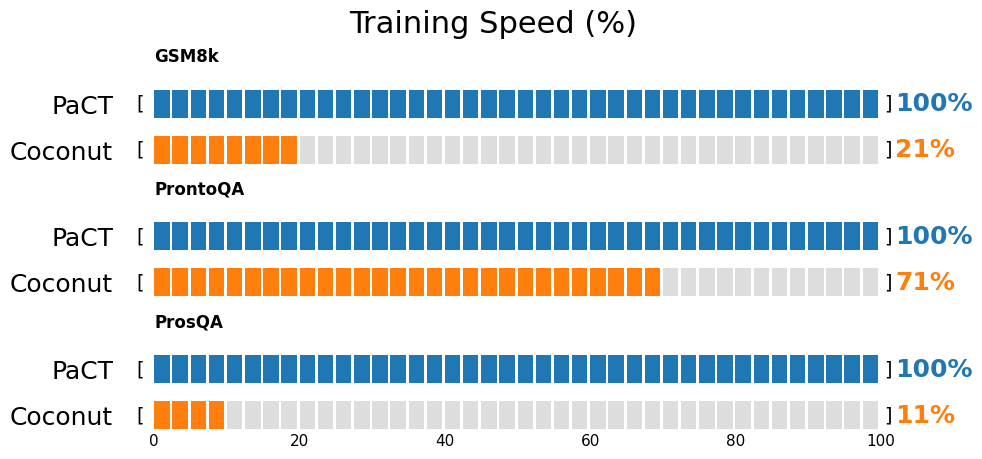
\includegraphics[width=\linewidth]{imgs/intro_diagram.png}
%   \caption{PaCT vs Coconut- training speed.}
%   \label{fig:concept_diagram_intro}
% \end{figure}

% Large language models (LLMs) have recently demonstrated impressive multi-step reasoning capabilities when prompted to generate explicit chains of thought (CoT), in which intermediate reasoning steps are expressed as natural language tokens before producing a final answer \cite{paper11}. While effective, this paradigm tightly couples reasoning to the discrete token space of language, forcing models to externalize internal computation through sequential text generation. This coupling introduces fundamental limitations: Language tokens are optimized for communication, not for the core needs of reasoning such as abstraction, conceptualization, and computation. Moreover, autoregressive decoding commits to a single partial trajectory token-by-token, and the compute cost grows linearly with the number of generated tokens \cite{paper14}. These shortcomings make detailed reasoning expensive and sub-optimal.
% %language tokens are optimized for communication rather than computation, autoregressive decoding enforces premature commitment to individual reasoning paths, and reasoning cost scales linearly with the number of generated tokens \cite{paper14}.

% A large body of work has sought to mitigate these issues through improved prompting strategies and decoding-time search. Approaches such as decomposed prompting \cite{paper12}, least-to-most prompting \cite{paper13}, self-consistency and beam-style decoding \cite{paper16}, and tree-based search over reasoning trajectories \cite{paper15} improve reliability by exploring or aggregating multiple textual reasoning paths. However, these methods still operate entirely in token space and inherit its core sequential bottleneck: each reasoning step must be generated, evaluated, and committed one token at a time. As a result, these methods primarily improve exploration in the same substrate rather than enabling more abstract or information-dense internal computation.
% %As a result, improvements come primarily from better exploration strategies rather than from changes to the underlying computational substrate.

% %This motivates moving reasoning off the discrete token stream and into the model’s continuous hidden-state space.
% Recent work has therefore explored shifting reasoning from explicit language tokens into the model’s continuous hidden state space. \emph{Chain of Continuous Thought} (Coconut) introduced a simple but powerful idea: replace segments of the textual chain-of-thought with continuous latent representations that are never decoded as language, and train them implicitly via their effect on the final answer likelihood \cite{paper1}. Empirically, Coconut demonstrates that models trained in this manner can exhibit emergent search behaviors resembling breadth-first exploration, while requiring fewer explicit reasoning tokens.

% Theoretical analysis has since clarified why continuous latent reasoning can be fundamentally more expressive than discrete CoT. \emph{Reasoning by Superposition} proves that continuous latent thoughts can represent superpositions of multiple candidate reasoning states simultaneously, enabling parallel exploration within a single latent step \cite{paper3}. In contrast, discrete token-based reasoning necessarily collapses this superposition into a single path at each decoding step, leading to inherently sequential exploration. These results establishes a formal expressivity gap between continuous and discrete reasoning mechanisms and provide a theoretical foundation for Coconut-style latent reasoning.

% Despite its promise, Coconut’s original formulation suffers from a critical limitation. Continuous thoughts are generated \emph{sequentially}: each latent vector is produced by feeding the previous hidden state back as the next input embedding, effectively introducing a recurrent unrolling inside the Transformer \cite{paper1}. This design reinstates an RNN-like dependency structure, causing the critical path length to grow linearly with the number of latent steps. Due to autoregressive nature, which prevents Coconut to reason deeply deeply in multiple stages. This scaling challenge prevent Coconut to fully leverage abstract thinking, weakening the very benefit latent representations are meant to provide.
% %despite being conceptually addressed by latent token inclusion. 
% As a result, training becomes substantially slower, hardware parallelism is poorly utilized, and optimization stability degrades as latent depth or model size increases.

% Several recent methods attempt to address efficiency concerns within latent reasoning. In particular, CoLaR \cite{paper2} proposes dynamically compressing chains of thought into fewer latent steps and optimizes the compression policy using reinforcement learning to trade off reasoning length and accuracy. CoLaR’s latent representations are explicitly supervised to preserve token-level semantics and are trained to reconstruct compressed textual reasoning segments. While effective for reducing the number of latent steps, this design retains autoregressive latent unrolling and constrains latents to remain semantically aligned with surface-level language. As a result, CoLaR primarily accelerates reasoning by compressing existing token-based trajectories, rather than altering the underlying computational structure of latent reasoning or enabling internal reorganization of reasoning dynamics. Consequently, it does not remove the core sequential dependency inherent in recurrent latent unrolling.


% In this work, we introduce \emph{Parallel Continuous Thought} (PaCT), a reformulation of continuous latent reasoning that eliminates recurrent latent unrolling altogether (Figure \ref{fig:PaCT_module}). Instead of generating latent thoughts sequentially, PaCT synthesizes a set of latent representations \emph{in parallel} using a learnable codebook of query vectors and cross-attention to the current textual context. By re-synthesizing latents at each reasoning stage rather than recursively accumulating prior latent states, PaCT enables each stage to capture distinct, context-grounded reasoning information. These latents are further refined through bidirectional interaction within a latent workspace before conditioning subsequent decoding. This design not only decouples reasoning capacity from serial computation depth, yielding substantial efficiency gains, but also promotes more information-dense and stable latent representations (Figure 0), allowing fewer latent variables to support deeper and more effective reasoning.


% Empirically, PaCT matches or exceeds the reasoning accuracy of Coconut across diverse mathematical and logical reasoning benchmarks \cite{dataset1,dataset2,dataset3} and model scales while achieving 4--9$\times$ reductions in training time (Figure \ref{fig:concept_diagram_intro}). 
% Beyond efficiency, our analyses show that PaCT acheives more information-rich latent reasoning: (i) fewer latent variables can achieve comparable or better accuracy than recurrent latent unrolling, (ii) increasing latent depth yields consistent gains without requiring increased latent width, and (iii) successive stages encode distinct, context-grounded information rather than redundantly accumulating latent history.
% %PaCT demonstrates improved latent quality: models trained with fewer latent variables achieve comparable or better performance than recurrent latent unrolling, and increasing reasoning depth yields consistent gains without increasing latent width. Analysis of latent representations shows that successive PaCT stages capture distinct, context-grounded reasoning information rather than redundantly accumulating latent history. 
% %Together, these results establish that parallel latent synthesis is not merely an acceleration strategy, but an architectural improvement that enables more information-dense, stable, and scalable continuous latent reasoning.
% Following are the our main contributions - 
% \begin{itemize} \itemsep0pt \parsep0pt \topsep2pt
%     \item \textbf{Parallel latent reasoning without recurrent unrolling.}
%     We introduce parallelism at the latent-token level by eliminating recurrent latent unrolling, and enable deeper reasoning at scale through a novel latent reasoning mechanism, called as PaCT that synthesizes latent tokens in parallel using learnable codebook queries and cross-attention to the textual context; this yields substantially faster training while achieving state-of-the-art reasoning accuracy (Figure \ref{fig:PaCT_module}).

%     \item \textbf{Information-rich latents via within-stage deliberation.}
%     %We introduce a \emph{bidirectional latent deliberation workspace} that refines synthesized latents within each stage, producing more information-dense latent states and supporting deeper reasoning \emph{without increasing latent width}.
%     We make latent tokens more information-rich by introducing bidirectional latent deliberation within each reasoning stage, improving latent reasoning capacity without increasing latent width (Figure \ref{fig:bidirectional_self_attention}).

% \end{itemize}


\section{Introduction}

\begin{figure}[h!]
  \centering
  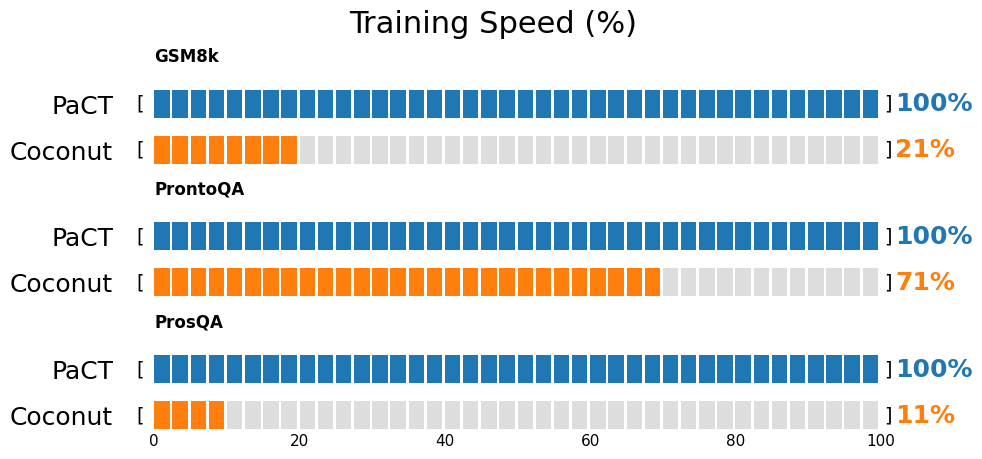
\includegraphics[width=\linewidth]{imgs/intro_diagram.png}
  \caption{PaCT vs Coconut- training speed.}
  \label{fig:concept_diagram_intro}
\end{figure}

Large language models (LLMs) have recently demonstrated impressive multi-step reasoning capabilities when prompted to generate explicit chains of thought (CoT), in which intermediate reasoning steps are expressed as natural language tokens before producing a final answer \cite{wei2022chain}. While effective, this paradigm tightly couples reasoning to the discrete token space of language, forcing models to externalize internal computation through sequential text generation. This coupling introduces fundamental limitations: Language tokens are optimized for communication, not for the core needs of reasoning such as abstraction, conceptualization, and computation \cite{fedorenko2024language,amalric2019distinct,monti2007functional,monti2009boundaries,monti2012thought,fedorenko2011functional}. Moreover, autoregressive decoding commits to a single partial trajectory token-by-token, and the compute cost grows linearly with the number of generated tokens \cite{saparov2022language}. These shortcomings make detailed reasoning expensive and sub-optimal.

A large body of work has sought to mitigate these issues through improved prompting strategies and decoding-time search. Approaches such as decomposed prompting \cite{khot2022decomposed}, least-to-most prompting \cite{zhou2022least}, self-consistency and beam-style decoding \cite{xie2023self}, and tree-based search over reasoning trajectories \cite{yao2023tree} improve reliability by exploring or aggregating multiple textual reasoning paths. Related work has also explored adding test-time deliberation signals that encourage models to ``think'' before committing to an output \cite{zelikman2024quiet}. However, these methods still operate entirely in token space and inherit its core sequential bottleneck: each reasoning step must be generated, evaluated, and committed one token at a time. As a result, these methods primarily improve exploration in the same substrate rather than enabling more abstract or information-dense internal computation.

Recent work has therefore explored shifting reasoning from explicit language tokens into the model’s continuous hidden state space. \emph{Chain of Continuous Thought} (Coconut) introduced a powerful idea to replace segments of the textual chain-of-thought with continuous latent representations that are never decoded as language, and train them implicitly via their effect on the final answer likelihood \cite{hao2024training}. Empirically, Coconut demonstrates that models trained in this manner can exhibit emergent search behaviors resembling breadth-first exploration, while requiring fewer explicit reasoning tokens.

Theoretical analysis has since clarified why continuous latent reasoning can be fundamentally more expressive than discrete CoT. \emph{Reasoning by Superposition} proves that continuous latent thoughts can represent superpositions of multiple candidate reasoning states simultaneously, enabling parallel exploration within a single latent step \cite{zhu2025reasoning}. In contrast, discrete token-based reasoning necessarily collapses this superposition into a single path at each decoding step, leading to inherently sequential exploration. These results establish a formal expressivity gap between continuous and discrete reasoning mechanisms and provide a theoretical foundation for Coconut-style latent reasoning.

Despite its promise, Coconut’s original formulation suffers from a critical limitation. Continuous thoughts are generated \emph{sequentially}: each latent vector is produced by feeding the previous hidden state back as the next input embedding, effectively introducing a recurrent unrolling inside the Transformer \cite{hao2024training}. This design reinstates an RNN-like dependency structure, causing the critical path length to grow linearly with the number of latent steps. Due to autoregressive nature, which prevents Coconut to reason deeply deeply in multiple stages. This scaling challenge prevent Coconut to fully leverage abstract thinking, weakening the very benefit latent representations are meant to provide. As a result, training becomes substantially slower, hardware parallelism is poorly utilized, and optimization stability degrades as latent depth or model size increases.

Several recent methods attempt to address efficiency concerns within latent reasoning. In particular, CoLaR \cite{tan2025think} proposes dynamically compressing chains of thought into fewer latent steps and optimizes the compression policy using reinforcement learning to trade off reasoning length and accuracy. CoLaR’s latent representations are explicitly supervised to preserve token-level semantics and are trained to reconstruct compressed textual reasoning segments. While effective for reducing the number of latent steps, this design retains autoregressive latent unrolling and constrains latents to remain semantically aligned with surface-level language. As a result, CoLaR primarily accelerates reasoning by compressing existing token-based trajectories, rather than altering the underlying computational structure of latent reasoning or enabling internal reorganization of reasoning dynamics. Consequently, it does not remove the core sequential dependency inherent in recurrent latent unrolling.

In this work, we introduce \emph{Parallel Continuous Thought} (PaCT), a reformulation of continuous latent reasoning that eliminates recurrent latent unrolling altogether (Figure \ref{fig:PaCT_module}). Instead of generating latent thoughts sequentially, PaCT synthesizes a set of latent representations \emph{in parallel} using a learnable codebook of query vectors and cross-attention to the current textual context. By re-synthesizing latents at each reasoning stage rather than recursively accumulating prior latent states, PaCT enables each stage to capture distinct, context-grounded reasoning information. These latents are further refined through bidirectional interaction within a latent workspace before conditioning subsequent decoding. This design not only decouples reasoning capacity from serial computation depth, yielding substantial efficiency gains, but also promotes more information-dense and stable latent representations (Figure~\ref{fig:concept_diagram_intro}), allowing fewer latent variables to support deeper and more effective reasoning.

Empirically, PaCT matches or exceeds the reasoning accuracy of Coconut across diverse mathematical and logical reasoning benchmarks \cite{dataset1,dataset2,dataset3} and model scales while achieving 4--9$\times$ reductions in training time (Figure \ref{fig:concept_diagram_intro}). 
Beyond efficiency, our analyses show that PaCT acheives more information-rich latent reasoning: (i) fewer latent variables can achieve comparable or better accuracy than recurrent latent unrolling, (ii) increasing latent depth yields consistent gains without requiring increased latent width, and (iii) successive stages encode distinct, context-grounded information rather than redundantly accumulating latent history.

Following are the our main contributions -
\begin{itemize} \itemsep0pt \parsep0pt \topsep2pt
    \item \textbf{Parallel latent reasoning without recurrent unrolling.}
    We introduce parallelism at the latent-token level by eliminating recurrent latent unrolling, and enable deeper reasoning at scale through a novel latent reasoning mechanism, called as PaCT that synthesizes latent tokens in parallel using learnable codebook queries and cross-attention to the textual context; this yields substantially faster training while achieving state-of-the-art reasoning accuracy (Figure \ref{fig:PaCT_module}).
    \item \textbf{Information-rich latents via within-stage deliberation.}
    We make latent tokens more information-rich by introducing bidirectional latent deliberation within each reasoning stage, improving latent reasoning capacity without increasing latent width (Figure \ref{fig:bidirectional_self_attention}).
\end{itemize}
